%
% File acl2020.tex
%
%% Based on the style files for ACL 2020, which were
%% Based on the style files for ACL 2018, NAACL 2018/19, which were
%% Based on the style files for ACL-2015, with some improvements
%%  taken from the NAACL-2016 style
%% Based on the style files for ACL-2014, which were, in turn,
%% based on ACL-2013, ACL-2012, ACL-2011, ACL-2010, ACL-IJCNLP-2009,
%% EACL-2009, IJCNLP-2008...
%% Based on the style files for EACL 2006 by 
%%e.agirre@ehu.es or Sergi.Balari@uab.es
%% and that of ACL 08 by Joakim Nivre and Noah Smith

\documentclass[11pt,a4paper]{article}
\usepackage[hyperref]{acl2020}
\usepackage{times}
\usepackage{amssymb}
\usepackage{amsmath}
\usepackage{float}
\usepackage{latexsym}
\usepackage{graphicx}
\usepackage{caption}
\usepackage{subcaption}
\usepackage{booktabs}
\renewcommand{\UrlFont}{\ttfamily\small}

% This is not strictly necessary, and may be commented out,
% but it will improve the layout of the manuscript,
% and will typically save some space.
\usepackage{microtype}

\aclfinalcopy % Uncomment this line for the final submission
%\def\aclpaperid{***} %  Enter the acl Paper ID here

%\setlength\titlebox{5cm}
% You can expand the titlebox if you need extra space
% to show all the authors. Please do not make the titlebox
% smaller than 5cm (the original size); we will check this
% in the camera-ready version and ask you to change it back.

\newcommand\BibTeX{B\textsc{ib}\TeX}

\title{Another (Ensemble) Transformer-Based Recommendation Model on Users-Items Interaction using Reviews}

\author{Triaji Wicaksono \\
  UC Berkeley \\
  \texttt{aji.wicaksono@berkeley.edu} \\\And
  Sean Campos \\
  UC Berkeley \\
  \texttt{sean.campos@berkeley.edu} \\}

\date{}



\graphicspath{{./images/}}

\begin{document}
\maketitle
\begin{abstract}
Recommendation systems typically come in two forms: Collaborative Filtering (similarity between users' preferences) and Content-Based Filtering (comparison between the properties of the items and users profile), however both of these approaches leave out the valuable information contained in user sourced reviews. We introduce an Ensemble Transformer Model producing users and items review embeddings that are well suited for recommendation tasks. We propose the Two-tower BERT\textsubscript{BASE} model as our baseline model, and incrementally augment that with Transformer model(s) performing the ensemble technique\footnotemark. We evaluate both \emph{feature-based} on different poolings and \emph{fine-tuning} strategies to learn latent feature representation of users and items reviews performing such downstream tasks. Additionally, we successfully feed our model with a highly dimension variant of number of users and items reviews, and obtain significant improvement over previous similar works using Convolutional Neural Networks.

\footnotetext{See our \href{https://github.com/sony-w/RecommendationTransformer}{Github repository}}
\end{abstract}

\section{Introduction}

As the number and diversity of products and services available to consumers increase at an escalating pace, especially in ever-growing online market places, it is becoming both increasingly important and challenging for consumers to discover and compare offerings. Hence, the recommendation system is becoming an essential part of purchasing decisions. Although the collaborative filtering approach has been highly successful, its crucial shortcoming is the cold start problem.  Collaborative filtering performs poorly when users or items have a relatively small ratings count as compared to the overall size of the catalogs, and since the numbers both users and items are only increasing, the threshold for overcoming that problem is rising.  One approach to mitigate this is to take advantage of the vast pool of information available in user generated reviews. As any online shopper can attest, reviews written by other customers contain a wealth of information, but their unstructured nature and large volume make them difficult to digest.  Up until recently these challenges have defied machine processing techniques, however recent advances are beginning to allow us to tap into their potential. 

Promising empirical results have already been achieved by \citet{zheng2017joint-modeling} and further refined by using a \citet{DeepCoNN-Movie}.  Both teams apply Deep Convolutional Neural Networks (DeepCoNN) to learn latent features separately for reviews written by each user and reviews written for each product, then those networks are combined to make a recommendation with improved accuracy.  We note that these approaches have seen significant performance improvements when different embedding techniques were utilized and see this as an opportunity for enhancement by using BERT and other transformer based approaches.


\section{Background}
The main focus of our experiments is to extend and enhance the  \citet{zheng2017joint-modeling} architecture by utilizing a variety of transformer based approaches with an emphasis on BERT in particular.  The specific task is to predict the rating that a user will give to a particular item by using two-tower network that learns hidden latent features for both users and items. One side of tower models user behavior by extracting semantic information from reviews written by the user, while simultaneously the other tower does the same using reviews for the item.  A shared layer on top of both of these towers then allows the latent factors to interact with each other, in an approach that follows from the core idea of matrix factorization, and is then used to make a rating prediction for a user-item pairing.

Previous works showed that larger GloVe embedding vectors and applying different pooling techniques to the resulting embedded sequences had potential for significant performance improvement.  We think that the BERT \citep{devlin2019bert} transformer based embedding vectors are very likely to outperform GloVe on this task. Additionally we are motivated by \citet{raghavendra-transformer-2019} whose result showed excellent performance from a relatively straightforward approach to pooling and a work by  \citet{fine-tune-bert-classification} on capturing features at different hidden states.

\subsection{Reviews Datasets}
We choose two real world datasets, Amazon product reviews and Yelp business reviews.  Yelp makes 8.6 million reviews from 160,585 businesses available for academic research purposes.  From this dataset, we choose 356,060 reviews with token lengths (as defined by the BERT uncased tokenizer) between 25 and 65.  We use a dataset of 3.4 million reviews from Movies and TV category on Amazon’s site provided by \citet{jianmo-amazon-dataset}.  We selected 171,854 reviews from this dataset using the same token length criteria.  The lower bound ensures that we have enough words to contain meaningful semantic information and the upper bound provides a reasonable limit of the required computational resources while capturing a significant proportion of the review texts (see Appendix~\ref{sec:appendix-review-lengths}), allowing us an opportunity to explore a larger number of configuration options in our experiments.  All of the users and items selected in each dataset have between 10 and 50 review texts in each group.  The lower bound is small enough to be problematic for matrix factorization approaches, allowing us to tackle the cold start problem.  The upper bound is large enough to demonstrate that our approach is not undermined by BERT's maximum sequence length of 512 tokens.

\section{Methods}

This section illustrates our modeling approach in detail to learn sequential user activities and item properties using reviews such that it estimates the rating given by users on items. It is achieved with two-tower Transformer based model and jointly coupled with a shared layer at the end resulting the ratings with minimum prediction error. We also describe how we process the dataset that highly differs in number of reviews dimension.

\subsection{Pre-Processing}
There are a few issues with our dataset that need to be addressed before we can begin feeding a sentence into a tokenizer.  First, the dataset contains some recording errors as well as spam entries.  The errors typically come in the form of an incomplete review, followed by the complete review in the subsequent row. To address this, we filter out all but the longest review for any single item by any single user.  The spam reviews typically contain the same phrases repeated over and over e.g. “This movie is great! This movie is great!”, so we eliminate those reviews with repeated sentences.

The other problem has to do with the size of the dataset we are working with.  We want our neural network to have access to all of the reviews that a user has written (excluding the review for the row that is currently being evaluated) as well as all of the reviews for an item (similarly, excluding the review that is being predicted) whenever it learns the features for each row of our dataset.  It means that different combinations of review text are repeated frequently.  Recomputing the complete BERT embedding vectors each time a review is needed by the model would be inefficient and require many days of processing time.  Storing the vectors for every contextualized token would require a significant amount of storage.  Our solution is to compute the embedding vectors for the entire reviews, then apply a pooling strategy to the sequence of the review vectors. We store the pooled vector in sorted order, perform lookup using fast binary tree index and efficiently group them into a single row.

\subsection{Two-tower Architecture}

The architecture of our model is a two-tower approach, with twin parallel networks, one for the users and the other one for the items.  The bottom of the  Figure \ref{fig:Architecture Diagram} starts with a lookup layer, where the text for each review is pulled from a cache and stacked respectively to the group of all the reviews for each user and all of the reviews for each item. The review written by the current user for the current item is omitted from this process to prevent the model from "seeing into the future".  On each side, the text then moves through a BERT layer to produce a matrix of embedding vectors with tokens as the columns and reviews as the rows within the grouping.

The next layers pool the embedding vectors across each review and the groups of reviews are then pooled together.  We explore a variety of pooling strategies for both of these steps which are detailed below.  In the final stage of each tower, the output from the pooling layers are considered features and passed into a fully connected dense layer with 32 nodes on each tower.

\begin{figure*}[t!]
     \centering
     \begin{subfigure}[b]{0.65\textwidth}
         \centering
         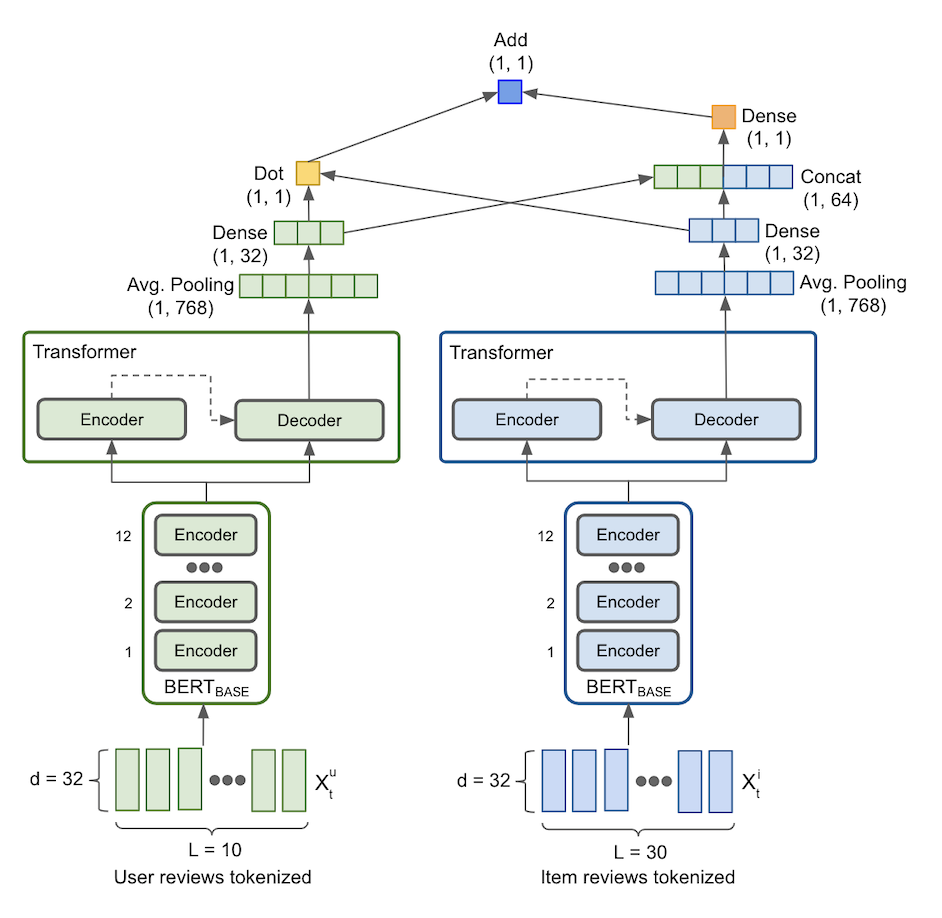
\includegraphics[width=\textwidth]{images/BERT+Transformer_Architecture_Diagram.png}
         \caption{BERT\textsubscript{BASE} + Transformer}
         \label{fig:f1}
     \end{subfigure}
     \hfill
     \begin{subfigure}[b]{0.3\textwidth}
         \centering
         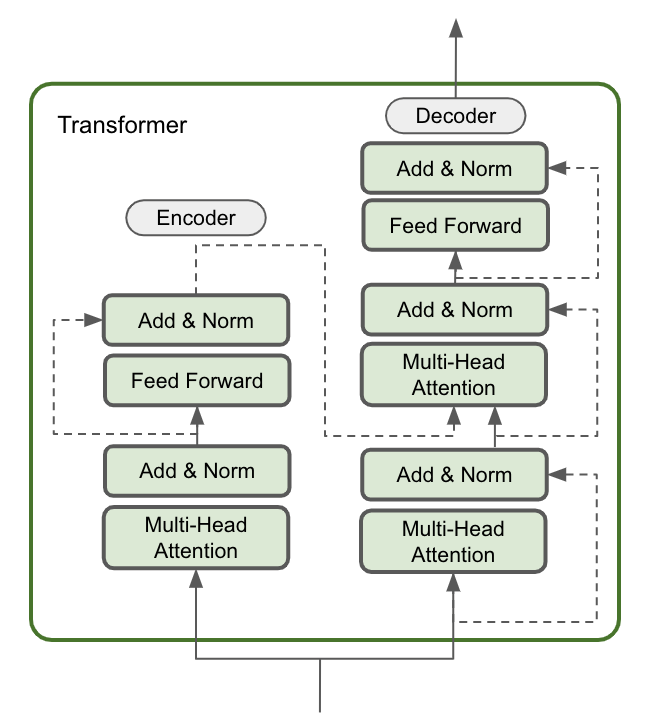
\includegraphics[width=\textwidth]{images/Transformer_Block.png}
         \caption{Transformer Block}
         \label{fig:f2}
     \end{subfigure}
        \caption{Architecture Diagram}
        \label{fig:Architecture Diagram}
\end{figure*}

\subsection{Shared Layer}

We use a similar shared layer technique introduced by \citet{zheng2017joint-modeling} to map the latent feature of users and items reviews into the same feature space. This models the interaction between the two, and therefore, we use this as the estimator of the corresponding rating motivated by Factorization Machine (FM) \citep{rendle2012factorization}. Due to the variant grouping dimension of our dataset, we first average the BERT sequence embeddings and concatenate $\bar{x}_u$ and $\bar{x}_i$ into a single vector $\hat{z} = (\bar{x}_u, \bar{x}_i)$. Given a batch of N training samples $\tau$, the cost function is calculated as Eq.\eqref{eq:interaction}.

\begin{equation}\label{eq:interaction}
    J = \hat{w_0} + \sum_{m=1}^{|\hat{z}|} \hat{w_m} \hat{z_m} + \sum_{m=1}^{|\hat{z}|} \sum_{n=m+1}^{|\hat{z}|} \langle \hat{v}_m, \hat{v}_n \rangle \hat{z}_m \hat{z}_n
\end{equation}

where $w_o \in \mathbb{R}$ is the global bias, $w \in \mathbb{R}^d$ denotes the weights of the $m_{th}$ variable in $\hat{z}$ and $\langle \hat{v}_m, \hat{v}_n \rangle$ denotes the second order interaction between $m_{th}$ and $n_{th}$ feature. The shared layer is then regularized with a 0.2 dropout.

\subsection{Fine-tuning}

For our experiment, we fine-tune a Two-tower BERT network and merge them with a shared layer. Let $\mathcal{U}$ be set of users, $\mathcal{I}$ be set of items, and $\mathcal{R}$ be set of ratings by the user $m$ to the item $n$, where $|\mathcal{U}| = M$, $|\mathcal{I}| = N$, and $|\mathcal{R}| = \{r_{m,n}\} \in \{1,2, \ldots, 5\}$. One side of the tower denotes $\mathcal{H}^u = (\mathcal{H}_1^u, \ldots, \mathcal{H}_n^u)$ as sequential of user interaction providing reviews on different items. Meanwhile the other side of the tower denotes a similar work of item-based Collaborative Filtering (CF) \citep{amjad-cf-2018}. Upon training, we use Adam optimizer with initial learning rate of $2e^{-6}$ and  \emph{ReduceLROnPlateau} callback of factor equals $0.2$ and patience is set to $5$.

\citet{raghavendra-transformer-2019} showed that using Transformer over BERT (ToBERT) benefits capturing better semantic representation over long sequences of text. We hence, ensemble our Two-tower BERT model with a two multi-head attention Transformer encoder-decoder as depicted on Figure.\ref{fig:Architecture Diagram}. We also experiment with few variants of Transformer, where we have a dual-stacked of Transformer (BERT\textsubscript{BASE} Two-tower + Bi-Transformer) and single Transformer with $n$ numbers of encoder-decoder (BERT\textsubscript{BASE} Two-tower + Deep Transformer). We need to be cautious for the selection of hyperparameters tuning so that we can fit our experiments into a single GPU Tesla P100-PCIE-16GB.

\subsection{Features-based on Different Poolings}

Following the works by \citet{devlin2019bert}, a feature-based approach, where fixed-embeddings are extracted from a pre-trained BERT model, has several virtues. Not all language modeling tasks can be easily represented, and therefore, adding a simple task-specific model architecture can better generalize performing such tasks. Our shared layer does exactly that. More importantly, there are major computational benefits to pre-compute an expensive representation of the training samples once and run many experiments with cheaper models. We experiment with many different combinations of pooling strategies within twelve hidden-state layers of BERT\textsubscript{BASE}. We are interested to see how different layers capture latent feature representation of users and items reviews for recommendation task.

\subsection{Evaluation}

We use the well known Mean Squared Error (MSE) metric, looking at the difference between our predicted product ratings and the user's actual rating, making our results comparable to collaborative filtering. To meet the top-N recommendations objective, this metric can be easily translated to binary problem to obtain recommended and relevant items by using \emph{precision and recall at k}, where \emph{k} is a pre-defined integer to match such top-N recommendations. However, this is not the focus of our experiments.

Table \ref{table:4} organizes each dataset to the number of ratings trained and tested on, as well as the size of the pool of reviews where groupings of review text are selected from.  As a reference point, we also compute an MSE using the average rating as the predicted rating and matrix factorization. Due to the limited time and resources, all of our experiments are run on the Amazon dataset, then selected models are run on the Yelp dataset for comparison.

\begin{table}[H]
\centering
\small
\begin{tabular}{@{} l *2r @{}}
\cline{2-3}
\multicolumn{1}{l}{\textbf{}} & \textbf{Amazon} & \textbf{Yelp}  \\ 
\midrule
 Count of Training Ratings & 20,000 & 32,500 \\ 
 Count of Testing Ratings & 2,000 & 3,200 \\
 Review Texts in Training Pool & 100,000 & 230,000 \\
 Count of Held Out Test Ratings & 5,300 & 14,000 \\
 Reviews in Held Out Testing Pool & 70,000 & 115,000 \\
 MSE from Matrix Factorization & 1.05 & 1.01 \\
\bottomrule
\end{tabular}
\caption{Pre-Trained Model Comparison}
\label{table:4}
\end{table}

\section{Results and Discussion}

We frame our experiments around examining four aspects of applying transformers to our recommendation task.  First, comparing different approaches to pooling the encoded BERT embeddings, as large transformer models are resource intensive to train, these strategies will be essential in designing a practical real word solution.  Second, comparing several variations of the pre-trained BERT transformer models. Third, fine-tuning BERT models specifically for our task and architecture.  Finally, comparing selected models with the Yelp dataset to examine the generalizability of our results.

\subsection{Baseline}

Our baseline architecture and strategy is BERT\textsubscript{BASE} uncased as our transformer encoding layer, and for a pooling strategy we use the mean of all the regular token embeddings (meaning we excluded the {\fontfamily{pcr}\selectfont[CLS]} and {\fontfamily{pcr}\selectfont[SEP]} special tokens) from the second-to-last hidden state, and then take the mean of the resulting embeddings across each of the reviews in the group. Our initial baseline result of 0.94 demonstrates that our proposed architecture can provide significant improvements over traditional collaborative filtering method, which scored 1.05 and over the \citet{zheng2017joint-modeling} model which scored 1.34 on this dataset.

\subsection{Pooling Strategy Results}

We use BERT\textsubscript{BASE} uncased to generate the embedding vectors for each of these experiments, and the result for each pooling strategy are in Table \ref{table:1}.  At the sequence level, mean pooling refers to averaging the embedding vectors across all the regular token embeddings (excluding {\fontfamily{pcr}\selectfont[CLS]} and {\fontfamily{pcr}\selectfont[SEP]}), and max pooling is the maximum of these vectors.  When embeddings are concatenated, a single vector with twice the width of a normal embedding is produced. At the group level, mean pooling refers to averaging the sequence-pooled vectors for each review in the group, max is the maximum pooled sequence across all of the reviews, and sum adds all the pooled vectors together.  Attentive pooling uses additive attention formula \citep{bahdanau-2015} to produce a weighted average for each sequence of embedding vectors. 

\begin{table*}[t!]
\centering
\small
\begin{tabular}{@{} *3l r l @{}}
\toprule
\multicolumn{1}{l}{\textbf{Sequence Pool}} & \textbf{Group Pool} & \textbf{Layers} & \textbf{Seq-Len} & \textbf{MSE}  \\ 
\midrule
 Mean & Mean & Second-to-Last Hidden & 64 & 0.94 \\ 
 Mean & Mean & Second-to-Last Hidden & 128 & \textcolor[rgb]{0.098,0.098,0.098}{0.97} \\
 Mean & Mean & Last Hidden & 128 & 1.17 \\
 Mean & Mean & Sum Last Four Hidden  & 128 & 0.92 \\
 Mean & Mean & Sum All 12 & 128 & \textbf{0.91} \\
 Mean & Max & Second-to-Last Hidden & 64 & 0.97 \\
 Mean & Sum & Second-to-Last Hidden & 64 & 1.04 \\
 Max & Mean & Second-to-Last Hidden & 64 & 0.95 \\
 Max & Max & Second-to-Last Hidden & 64 & 0.97 \\
 Concat Max Mean & Mean & Second-to-Last Hidden & 64 & 0.93 \\
 Mean & Mean & Concat Last 4 & 64 & 0.96 \\
 Mean & Mean & Concat Last 4 & 64 & 0.96 \\
\bottomrule
\end{tabular}
\caption{Pooling Strategy Results}
\label{table:1}
\end{table*}

The baseline model ranks reasonably high given the simplicity of taking the average across both axis of embedding vectors.  We believe that this relates to our choice of applying these operations to individually encoded review texts, which is an enhancement afforded to us by the advances in transformer architecture.  In prior works, the reviews text were concatenated into a single long string, however our approach maintains the positional information encoded into each vector as goes into the pooling operation.

The strategies that performed better than baseline included summing vectors across multiple layers or concatenating multiple pooling strategies, which suggests that better performance is gained by giving the pooling strategy access to more information.   

\subsection{BERT Model Variations}

We also examine how different variations on the BERT model perform at our recommendation task.  Since training a transformer model is resource intensive, it is useful to have a quantitative comparison of how pre-trained model choice effects performance.  

The results in Table \ref{table:2} below use the baseline mean-mean pooling strategy for consistency.

\begin{table}[H]
\centering
\small
\begin{tabular}{@{} l c @{}}
\toprule
\multicolumn{1}{l}{\textbf{Model}}    & \textbf{MSE}  \\ 
\midrule
 BERT\textsubscript{BASE} \citep{devlin2019bert} & 0.94 \\ 
 BERT\textsubscript{LARGE} & 0.95 \\
 RoBERTa \citep{liu2019roberta} & \textbf{0.91} \\
 DistilBERT \citep{sanh2020distilbert} & 1.01 \\
 SentenceBERT \citep{reimers2019sentencebert}  & 1.21 \\
 Universal Sentence Encoder \citep{cer2018universal}  & 0.95 \\
 Electra\textsubscript{BASE} \citep{clark2020electra} & 0.92 \\
\bottomrule
\end{tabular}
\caption{Pre-Trained Model Comparison}
\label{table:2}
\end{table}

Although many of the pre-trained models are competitive with each other, RoBERTa's performance stands out and we believe this is related to the text it is trained on.  Reviews authored by customers do not go through an editing process, and are typically not as linguistically correct as the writing typically seen in books or on Wikipedia.  We believe that RoBERTa benefits from having been trained with common crawl text in this respect.  Electra may also be handling this text better having been trained as a discriminator. Meanwhile, Universal Sentence Encoder performs closely to BERT\textsubscript{BASE} and in fact, similar to BERT\textsubscript{LARGE} with simpler architecture. We believe it has similar benefits to RoBERTa based on the fact that it was pre-trained on variety of data sources including discussion forums. 

SentenceBert is an interesting model to look at because it has sequence-level pooling built in and also uses a dot product in its Siamese architecture. However, our model intends to learn latent features from the reviews, so it should not be trying to find similarities in the sentences, therefore our hypothesis is that this model should perform poorly in comparison to the others and validates the idea that we are indeed learning features about the products and not just looking for similar sentences.

\subsection{Fine-tuning}

Our fine-tuning strategy with downstream task and domain data shows promising performance with much reduced tokens sequence length of 32. Compute resource constraint is our main consideration for this sequence length selection. The Two-tower BERT\textsubscript{BASE} alone results MSE of 0.95 and it outperforms \citet{zheng2017joint-modeling} with DeepCoNN architecture by $\approx29$\%. Ensembling that with another Transformer of encoder-decoder \citep{vaswani2017attention} results performance superior among our experiments with MSE of $0.90$ capturing better latent feature of users and items reviews interaction as seen in Table \ref{table:3}. However, with more complex model by using Bi-Transformer where there are dual-stack of identical Transformer or DeepTransformer where it contains $n$ number of encoders-decoders tend to display inferior results.

\begin{table}[H]
\centering
\small
\begin{tabular}{@{} l c @{}}
\toprule
\multicolumn{1}{l}{\textbf{Configuration}}    & \textbf{MSE}  \\ 
\midrule
 DeepCoNN & 1.34 \\ 
 BERT\textsubscript{BASE} Tower & 0.95 \\
 BERT\textsubscript{BASE} Tower + Transformer & \textbf{0.90} \\
 BERT\textsubscript{BASE} Tower + Bi-Transformer & \textbf{0.90} \\
 BERT\textsubscript{BASE} Tower + DeepTransformer (n=2) & 1.08 \\
 BERT\textsubscript{BASE} Tower + DeepTransformer (n=3) & 1.11 \\
\bottomrule
\end{tabular}
\caption{Fine-Tuning Results}
\label{table:3}
\end{table}

Fine-tuning is clearly a powerful solution when achieving the best possible performance, but it comes at an extremely steep computational resource cost.

\subsection{Generalizing to Other Datasets}

Our baseline model scores nearly identically between the Amazon and Yelp datasets, both with an MSE of 0.93, so it is certainly possible for our approach to generalize well.  However other model configuration options perform notably worse on the Yelp dataset (see Appendix~\ref{sec:appendix-yelp} for full results). This behavior also occurred in \citet{zheng2017joint-modeling}.  We believe this may be because the Yelp reviews are less focused and negative ratings often center on a specific incident and not reflective of the overall offering. A deeper examination could be performed as future work.


\section{Error Analysis}

We sample from the worst performing predictions in our held out test dataset and read through all the grouped reviews, as well as the ultimate rating and review given to by the user to the item to see if any patterns emerged.  Since this is only a sampling, the proportions reported below are meant to be rough estimates and not empirically measured.

In more than half of the worst predictions, the user's reaction was not predictable based on any information available in the review data.  Typically this was because there was a problem with the transaction and not the product itself.  In a few instances the user had no tolerance for a specific type of content, such as sexuality or violence, and this was not mentioned by other reviewers.  In about 20\% of the errors, the user simply disagreed with all of the other reviews, for example finding the movie boring when many users enjoyed it. There was a similar proportion where the reviews contained unusual entries, such as entire filmographies of the actors or related products.  In a real world environment these would likely be pre-filtered as spam or otherwise ineligible reviews.  Finally, there was a small category that appeared to be mis-clicks, for example leaving a positive description for a one-star review. 

\section{Conclusion}

User generated product reviews contain a wealth of information that has been inaccessible to recommender systems due to the unstructured nature of the content until now.  We have demostrated that Transformer based architectures can successfully mine information contained within review text to outperform matrix factorization approaches when faced with the cold start problem.  We offer a comparison of pooling techniques and pre-trained model choices which are less costly than fine-tuning a transformer model.  We also demonstrate that the best results can be achieved through fine-tuning, even with short text sequences.  Finally, we show that it is possible for these approaches to generalize to other domains.

Future research would include measuring the performance of the different pooling strategies against the different model variations and further exploring why certain models have degraded performance on the Yelp dataset.


\bibliography{recommender}
\bibliographystyle{acl_natbib}


\clearpage
\appendix
\section{Appendices}

\subsection{Tokens Length}
Based on the distribution histogram below, it shows that $\approx90$\% of the review tokens length falls between 25 and 65 tokens. Hence, it allows us to include majority of the reviews without compromising our model performance and yet we are still able to obtain reviews with more semantically meaningful.
\label{sec:appendix-review-lengths}
\begin{figure}[h]
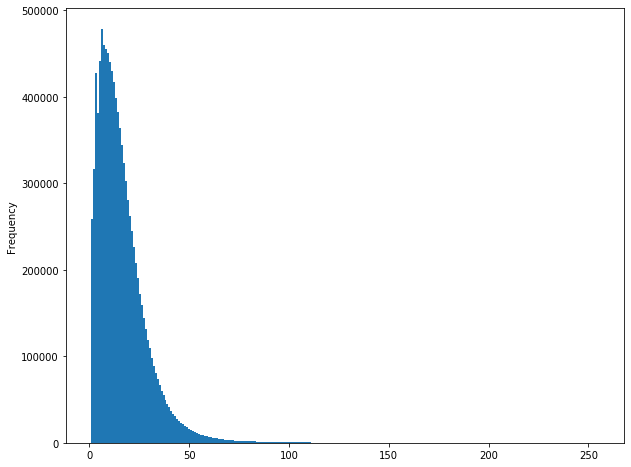
\includegraphics[width=20em]{images/token_length_hist.png}
\caption{Distribution of review text lengths}
\end{figure}

\subsection{Amazon and Yelp Comparison}
Our baseline model performs similarly well on both, however the other options have degraded performance on the Yelp dataset. Similar behaviors were demonstrated on DeepCoNN as well and this may require further investigation. We reason that the language used in Amazon dataset for reviewing Movies and TV might be considerably more consistent than in Yelp for reviewing businesses.
\label{sec:appendix-yelp}

\begin{table}[h]
\centering
\small
\begin{tabular}{@{} l r l *2r @{}}
\toprule
\multicolumn{1}{l}{\textbf{Model}} & \textbf{Seq-Len} & \textbf{Pooling Strategy / Fine-tuning} & \textbf{Amazon} & \textbf{Yelp}  \\ 
\midrule
 BERT\textsubscript{BASE} & 128 & Mean 2nd-to-Last Layer & 0.97 & 1.11 \\ 
 BERT\textsubscript{BASE} & 128 & Sum Last 4 Hidden & 0.92 & 1.08 \\
 BERT\textsubscript{BASE} & 64 & Mean 2nd-to-Last Hidden & 0.94 & 0.94 \\
 BERT\textsubscript{BASE} & 64 & Concat Mean + Max 2nd-to-Last Hidden & 0.93 & 0.95 \\
 RoBERTa & 64 & Mean 2nd-to-Last Layer & 0.91 & 0.94 \\
 BERT\textsubscript{BASE} Two-tower & 64 & Fine-tuning & 0.95 & 1.08 \\
 BERT\textsubscript{BASE} Two-tower + Transformer & 32 & Fine-tuning & 0.90 & 1.08 \\
 BERT\textsubscript{BASE} Two-tower + Bi-Transformer & 32 & Fine-tuning & 0.90 & 1.09 \\
 BERT\textsubscript{BASE} Two-tower + DeepTransformer (n=2) & 32 & Fine-tuning & 1.08 & 1.08 \\
 BERT\textsubscript{BASE} Two-tower + DeepTransformer (n=3) & 32 & Fine-tuning & 1.12 & 1.07 \\
\bottomrule
\end{tabular}
\caption{Performance comparison on Amazon vs Yelp datasets}
\end{table}


\end{document}
